%%%%%%%%%%%%%%%%%%%%%%%%%%%%%%%%%%%%%%%%%%%%%%%%%%%%%%%%%%%%%%%%%%%%%%%%
%% PhysMDT: Masked Diffusion Transformer for Physics Equation Derivation
%% Target venue: NeurIPS / Nature-class
%%%%%%%%%%%%%%%%%%%%%%%%%%%%%%%%%%%%%%%%%%%%%%%%%%%%%%%%%%%%%%%%%%%%%%%%
\documentclass[11pt,a4paper]{article}

%% ---- packages ----
\usepackage[margin=1in]{geometry}
\usepackage{amsmath,amssymb,amsfonts}
\usepackage{algorithm}
\usepackage{algorithmic}
\usepackage{booktabs}
\usepackage{hyperref}
\usepackage[round]{natbib}
\usepackage{pgfplots}
\pgfplotsset{compat=1.18}
\usepackage{tikz}
\usetikzlibrary{positioning,arrows.meta,shapes.geometric,fit,calc,decorations.pathreplacing}
\usepackage{subcaption}
\usepackage{multirow}
\usepackage{xcolor}
\usepackage{graphicx}
\usepackage{float}
\usepackage{enumitem}

%% colour palette (consistent throughout)
\definecolor{physblue}{HTML}{2E6DA4}
\definecolor{physorange}{HTML}{E67E22}
\definecolor{physgreen}{HTML}{27AE60}
\definecolor{physred}{HTML}{C0392B}
\definecolor{physpurple}{HTML}{8E44AD}
\definecolor{physgray}{HTML}{7F8C8D}

\hypersetup{
  colorlinks=true,
  linkcolor=physblue,
  citecolor=physblue,
  urlcolor=physblue
}

%% ---- macros ----
\newcommand{\PhysMDT}{\textsc{PhysMDT}}
\newcommand{\bx}{\mathbf{x}}
\newcommand{\by}{\mathbf{y}}
\newcommand{\bmask}{[\textsc{mask}]}
\newcommand{\R}{\mathbb{R}}
\newcommand{\E}{\mathbb{E}}

\title{%
  \textbf{\PhysMDT{}: A Masked Diffusion Transformer \\
  for Deriving Newtonian Physics Equations \\
  from Observational Data}}
\author{%
  Research Lab (Automated)%
}
\date{}

%% ====================================================================
\begin{document}
\maketitle

%% --------------------------------------------------------------------
%% ABSTRACT
%% --------------------------------------------------------------------
\begin{abstract}
Deriving symbolic physics equations from raw numerical observations remains a
central challenge at the intersection of machine learning and scientific
discovery.  We present \PhysMDT{}, a masked diffusion transformer that
reformulates equation derivation as iterative denoising: starting from a
fully masked token sequence, the model progressively reveals equation tokens
conditioned on numerical observation pairs.  Inspired by the first-place ARC
2025 ARChitects solution---which demonstrated that masked diffusion models
outperform autoregressive approaches on complex pattern-completion tasks---we
adapt four key innovations for the physics domain: (i) masked diffusion
training with variable masking ratios, (ii) iterative soft-mask refinement
with cold restarts for progressive equation unmasking, (iii) dual-axis
Rotary Position Embeddings encoding both sequence position and expression
tree depth, and (iv) test-time finetuning with LoRA for per-instance
adaptation.  We further incorporate physics-informed loss terms (dimensional
consistency, conservation regularisation, symmetry awareness) and a dual-model
architecture in which a lightweight structure predictor forecasts the equation
skeleton before the main model fills in variables and constants.  We evaluate
on a procedurally generated corpus of 61 Newtonian equation templates spanning
seven physics families and three difficulty levels, as well as the AI~Feynman,
Nguyen, and Strogatz benchmarks.  Our ablation study over eight architectural
variants and a refinement-depth study characterise the
quality--compute trade-off and identify architectural components that yield
the largest gains.  Although limited by CPU-scale training (d\_model=128, 1\,000
samples), \PhysMDT{} single-pass decoding achieves a 2.1$\times$ composite
score improvement over a matched autoregressive baseline and produces
equations of lower structural complexity, demonstrating the viability of
masked diffusion for symbolic physics derivation.
\end{abstract}

%% --------------------------------------------------------------------
%% 1  INTRODUCTION
%% --------------------------------------------------------------------
\section{Introduction}
\label{sec:intro}

The automated derivation of governing equations from observational data is a
long-standing aspiration of computational physics.  Given a set of
measurements $\{(x_i, y_i)\}_{i=1}^{N}$ sampled from an unknown physical law
$y = f(x)$, the goal is to recover the closed-form symbolic expression for
$f$.  This problem---\emph{symbolic regression}---has deep roots in genetic
programming~\citep{koza1994genetic} and has recently attracted intense interest
from the deep-learning community~\citep{lample2020deep,kamienny2022end,biggio2021neural,cranmer2023interpretable}.

Traditional evolutionary approaches such as PySR~\citep{cranmer2023interpretable}
search over combinatorial expression spaces using genetic operations.  While
effective for simple, low-variable equations, they struggle with the complex
multi-variable expressions prevalent in Newtonian mechanics---coupled
oscillators, Lagrangian formulations, and $N$-body gravitational
systems---due to exponential search-space growth~\citep{lacava2021srbench}.
Neural approaches have shown promise: \citet{lample2020deep} demonstrated that
sequence-to-sequence transformers can perform symbolic mathematics when
equations are treated as prefix-notation token sequences.  AI
Feynman~\citep{udrescu2020ai,udrescu2020ai2} combined neural networks with
physics-inspired decomposition heuristics.
NeSymReS~\citep{biggio2021neural} and ODEFormer~\citep{dascoli2023odeformer}
pushed transformer-based symbolic regression further.

All of the above neural methods employ \emph{autoregressive} (AR) decoding:
tokens are generated left-to-right, each conditioned only on its predecessors.
This sequential commitment is poorly matched to mathematical expressions,
which possess \emph{tree} structure and strong bidirectional constraints
(e.g., dimensional consistency, operator--operand compatibility).  A recent
breakthrough suggests a better paradigm: the ARC 2025 ARChitects
solution~\citep{arc2025architects}, which won the ARC-AGI-2 competition using
a masked diffusion model based on
LLaDA~\citep{nie2025llada}/MDLM~\citep{sahoo2024simple}.  Their key insight
is that \emph{iterative mask-and-predict} allows the model to reason
bidirectionally, revise earlier decisions, and progressively sharpen its
output---all properties highly desirable for equation derivation.

\paragraph{Contributions.}
We make the following contributions:
\begin{enumerate}[leftmargin=*,itemsep=2pt]
  \item \textbf{First application of masked diffusion to symbolic physics
        equation derivation.}  We introduce \PhysMDT{}, a bidirectional
        transformer trained with a masked diffusion objective on prefix-encoded
        physics equations conditioned on numerical observations
        (Section~\ref{sec:method}).
  \item \textbf{Adaptation of ARC-2025 techniques for scientific
        discovery.}  We transfer iterative soft-mask refinement with cold
        restarts, dual-axis Rotary Position Embeddings encoding expression
        tree depth, and test-time LoRA finetuning from the visual
        pattern-completion domain to symbolic mathematics
        (Sections~\ref{sec:refinement}--\ref{sec:ttf}).
  \item \textbf{Physics-informed regularisation.}  We augment the masked
        diffusion loss with dimensional consistency, conservation, and
        symmetry-awareness terms that inject domain knowledge without
        constraining the hypothesis space
        (Section~\ref{sec:physics_loss}).
  \item \textbf{Comprehensive empirical study.}  We present an ablation
        over eight architectural variants, a refinement-depth study, embedding
        space analysis, and evaluation on AI~Feynman, Nguyen, and Strogatz
        benchmarks (Section~\ref{sec:results}).
\end{enumerate}

The remainder of this paper is organised as follows.
Section~\ref{sec:related} reviews related work.
Section~\ref{sec:background} establishes notation and background.
Section~\ref{sec:method} details the \PhysMDT{} architecture and training
procedure.
Section~\ref{sec:setup} describes the experimental setup.
Section~\ref{sec:results} presents results and analysis.
Section~\ref{sec:discussion} interprets findings and discusses limitations.
Section~\ref{sec:conclusion} concludes.

%% --------------------------------------------------------------------
%% 2  RELATED WORK
%% --------------------------------------------------------------------
\section{Related Work}
\label{sec:related}

\paragraph{Transformers for symbolic mathematics.}
\citet{lample2020deep} pioneered the use of encoder--decoder transformers for
symbolic integration and differential equation solving, treating expressions
as prefix-notation token sequences.  \citet{kamienny2022end} extended this to
end-to-end symbolic regression from numerical data.  TPSR~\citep{sun2023tpsr}
combined transformers with Monte Carlo Tree Search for guided exploration.
ODEFormer~\citep{dascoli2023odeformer} targeted dynamical systems with
specialised architectures.

\paragraph{Physics-inspired equation discovery.}
AI Feynman~\citep{udrescu2020ai,udrescu2020ai2} exploits dimensional analysis,
symmetry, and separability to decompose the symbolic regression problem.
PINNs~\citep{raissi2019physics} incorporate differential-equation constraints
directly into neural network training---an approach we adapt through our
physics-informed loss terms.  PySR~\citep{cranmer2023interpretable} provides
a performant evolutionary search framework that achieves state-of-the-art on
the SRBench benchmark suite~\citep{lacava2021srbench}.

\paragraph{Masked diffusion models.}
LLaDA~\citep{nie2025llada} introduced large-scale masked diffusion for language
modelling, demonstrating competitive perplexity with autoregressive models.
MDLM~\citep{sahoo2024simple} showed that simple masked diffusion objectives
suffice for strong performance.  The ARC 2025
ARChitects~\citep{arc2025architects} applied LLaDA to the ARC-AGI challenge,
achieving first place with iterative soft-mask refinement, 2D positional
encoding, and test-time finetuning---techniques we adapt for equation
derivation.

\paragraph{LLMs for mathematical reasoning.}
Minerva~\citep{lewkowycz2022solving} and Llemma~\citep{azerbayev2024llemma}
demonstrated strong mathematical reasoning in large language models, primarily
through chain-of-thought prompting.  Our work differs in targeting
\emph{closed-form symbolic output} rather than natural-language solutions.

\paragraph{Symbolic regression benchmarks.}
The Nguyen benchmark~\citep{nguyen2011benchmark} provides 12 standard test
equations.  The Strogatz dataset~\citep{lacava2016strogatz} contains nonlinear
ODE systems.  SRBench~\citep{lacava2021srbench} offers a comprehensive
multi-method comparison.  We evaluate on all three plus AI~Feynman.

%% --------------------------------------------------------------------
%% 3  BACKGROUND & PRELIMINARIES
%% --------------------------------------------------------------------
\section{Background and Preliminaries}
\label{sec:background}

\paragraph{Symbolic regression.}
Given observations $\mathcal{D} = \{(\bx_i, y_i)\}_{i=1}^{N}$ where
$\bx_i \in \R^{d}$ and $y_i \in \R$, symbolic regression seeks a function
$\hat{f}$ from a hypothesis class $\mathcal{F}$ of closed-form expressions
that minimises a loss $\ell$ (typically MSE) subject to a complexity
regulariser:
\begin{equation}
  \hat{f} = \arg\min_{f \in \mathcal{F}} \;
    \sum_{i=1}^{N} \ell\!\bigl(f(\bx_i),\, y_i\bigr)
    + \lambda \cdot \text{complexity}(f).
  \label{eq:sr}
\end{equation}

\paragraph{Prefix notation.}
Following \citet{lample2020deep}, we encode mathematical expressions as token
sequences in Polish (prefix) notation.  For example, $\tfrac{1}{2}mv^2$ becomes
\texttt{[*~0.5~*~m~\^{}~v~2]}.  This representation is unambiguous without
parentheses and naturally maps to expression trees.

\paragraph{Masked diffusion.}
In the LLaDA framework~\citep{nie2025llada}, a forward process
$q(z_t \mid z_0)$ masks each token independently with probability $t$,
replacing it with a special \bmask{} token.  A neural network
$p_\theta(z_0 \mid z_t)$ is trained to reconstruct the original tokens at
masked positions.  The training objective is:
\begin{equation}
  \mathcal{L}_{\text{MDT}} =
    \E_{t \sim U(0,1)} \E_{z_t \sim q(z_t|z_0)}
    \left[-\sum_{i \in \mathcal{M}_t}
      \log p_\theta(z_0^{(i)} \mid z_t)\right]
  \label{eq:mdt_loss}
\end{equation}
where $\mathcal{M}_t$ is the set of masked positions at noise level $t$.

\paragraph{Rotary Position Embeddings (RoPE).}
RoPE~\citep{su2024roformer} encodes position through rotation matrices applied
to query--key pairs in attention.  For position $m$ and dimension pair
$(2i, 2i{+}1)$ with frequency $\theta_i = 10000^{-2i/d}$:
\begin{equation}
  \text{RoPE}(x, m) =
    \begin{pmatrix}
      x_{2i} \cos m\theta_i - x_{2i+1}\sin m\theta_i \\
      x_{2i} \sin m\theta_i + x_{2i+1}\cos m\theta_i
    \end{pmatrix}.
  \label{eq:rope}
\end{equation}

\paragraph{Notation summary.}
Table~\ref{tab:notation} summarises the key notation used throughout.

\begin{table}[h]
\centering
\caption{Summary of notation.}
\label{tab:notation}
\begin{tabular}{@{}ll@{}}
\toprule
\textbf{Symbol} & \textbf{Description} \\
\midrule
$\mathcal{D}$ & Observation dataset $\{(\bx_i, y_i)\}_{i=1}^{N}$ \\
$f$ & Ground-truth equation \\
$\hat{f}$ & Predicted equation \\
$z_0$ & Clean equation token sequence \\
$z_t$ & Partially masked sequence at noise level $t$ \\
$\mathcal{M}_t$ & Set of masked positions at level $t$ \\
$d_{\text{model}}$ & Transformer hidden dimension \\
$L$ & Number of transformer layers \\
$H$ & Number of attention heads \\
$V$ & Vocabulary size (155 tokens) \\
\bottomrule
\end{tabular}
\end{table}

%% --------------------------------------------------------------------
%% 4  METHOD
%% --------------------------------------------------------------------
\section{Method}
\label{sec:method}

\PhysMDT{} consists of five components: (1) an observation encoder, (2) a
bidirectional transformer with dual-axis RoPE, (3) a masked diffusion
training objective augmented with physics-informed losses, (4) an iterative
soft-mask refinement procedure for inference, and (5) auxiliary modules for
test-time finetuning (TTF), structure prediction, and token algebra.
Figure~\ref{fig:architecture} provides an overview.

\begin{figure}[t]
  \centering
  \includegraphics[width=\textwidth]{figures/architecture_diagram.png}
  \caption{\textbf{\PhysMDT{} architecture overview.}  Numerical observations
  $\{(x_i,y_i)\}$ are encoded by an MLP and cross-attended by the
  bidirectional transformer.  Equation tokens are embedded with dual-axis
  RoPE (sequence position + tree depth).  During training, random tokens are
  masked and the model predicts them via cross-entropy.  During inference, the
  iterative soft-mask refinement loop progressively unmasks the equation over
  $N$ refinement steps.}
  \label{fig:architecture}
\end{figure}

%% 4.1  Observation Encoder
\subsection{Observation Encoder}
\label{sec:obs_encoder}

Each observation pair $(x_i, y_i) \in \R^{d_\text{in}}$ is projected to the
model dimension via a two-layer MLP with GELU activation:
\begin{equation}
  h_i^{(\text{obs})} = W_2\,\text{GELU}(W_1[x_i;\, y_i] + b_1) + b_2,
  \quad h_i^{(\text{obs})} \in \R^{d_\text{model}}.
\end{equation}
These embeddings serve as keys and values for cross-attention in the
transformer blocks.

%% 4.2  Dual-Axis RoPE
\subsection{Dual-Axis Rotary Position Embeddings}
\label{sec:dual_rope}

Standard RoPE encodes only left-to-right sequence position.  Mathematical
expressions, however, have a natural \emph{hierarchical} structure: in the
prefix expression \texttt{[+~*~a~b~c]}, the root operator \texttt{+} is at
tree depth 0, while \texttt{a} and \texttt{b} are at depth 2.  Inspired by
the ARC 2025 solution's use of 2D RoPE for spatial grid
positions~\citep{arc2025architects}, we split the $d_\text{model}$ dimensions
into two halves:
\begin{itemize}[itemsep=2pt]
  \item \textbf{Axis 1} (dims $1\ldots d/2$): standard sequence position $m$.
  \item \textbf{Axis 2} (dims $d/2{+}1\ldots d$): expression tree depth
        $\delta(m)$, computed by counting prefix operators preceding
        position $m$.
\end{itemize}
Each axis applies the standard RoPE rotation (Eq.~\ref{eq:rope}) to its
respective dimension block.  This provides the model with an explicit
positional signal about the hierarchical level of each token, which is not
recoverable from content embeddings alone.

%% 4.3  Bidirectional Transformer
\subsection{Bidirectional Transformer Backbone}
\label{sec:transformer}

The core of \PhysMDT{} is a stack of $L$ transformer blocks, each containing:
\begin{enumerate}[itemsep=1pt]
  \item Multi-head self-attention (bidirectional---no causal mask).
  \item Multi-head cross-attention to observation encoder outputs.
  \item Feed-forward network with GELU activation.
\end{enumerate}
Unlike autoregressive decoders, every equation token position can attend to
\emph{all} other positions, enabling the model to exploit long-range
constraints (e.g., dimensional consistency between left- and right-hand sides).

%% 4.4  Masked Diffusion Training
\subsection{Masked Diffusion Training}
\label{sec:training}

Training follows the LLaDA protocol~\citep{nie2025llada}.  For each training
example $(z_0, \mathcal{D})$ where $z_0$ is the ground-truth equation token
sequence:
\begin{enumerate}[itemsep=1pt]
  \item Sample masking ratio $t \sim U(0, 1)$.
  \item For each position $j$, independently replace $z_0^{(j)}$ with
        \bmask{} with probability $t$, producing $z_t$.
  \item Compute cross-entropy loss over masked positions only
        (Eq.~\ref{eq:mdt_loss}).
\end{enumerate}

The variable masking ratio is critical: with $t$ near 0 the model sees
almost the full equation (learning local corrections), while with $t$ near 1
it must reconstruct the equation almost entirely from observations (learning
global structure).  This curriculum naturally emerges from the uniform
$t$-sampling.

Algorithm~\ref{alg:training} provides the complete training procedure.

\begin{algorithm}[t]
\caption{\PhysMDT{} Training}
\label{alg:training}
\begin{algorithmic}[1]
\REQUIRE Dataset $\{(z_0^{(k)}, \mathcal{D}^{(k)})\}_{k=1}^{K}$, model
$p_\theta$
\FOR{each mini-batch $\mathcal{B}$}
  \STATE $\mathcal{L} \gets 0$
  \FOR{$(z_0, \mathcal{D}) \in \mathcal{B}$}
    \STATE Sample $t \sim U(0,1)$
    \STATE $z_t \gets \text{MaskTokens}(z_0, t)$
    \hfill\COMMENT{Independently mask each position with prob $t$}
    \STATE $\hat{z}_0 \gets p_\theta(z_t, \;\text{Encode}(\mathcal{D}))$
    \STATE $\mathcal{L} \gets \mathcal{L} - \sum_{j \in \mathcal{M}_t}
           \log p_\theta(z_0^{(j)} \mid z_t,\, \mathcal{D})$
    \STATE $\mathcal{L} \gets \mathcal{L} + \lambda_\text{dim}\mathcal{L}_\text{dim}
           + \lambda_\text{cons}\mathcal{L}_\text{cons}
           + \lambda_\text{sym}\mathcal{L}_\text{sym}$
    \hfill\COMMENT{Physics losses (Sec.~\ref{sec:physics_loss})}
  \ENDFOR
  \STATE Update $\theta$ via AdamW on $\mathcal{L}/|\mathcal{B}|$
\ENDFOR
\end{algorithmic}
\end{algorithm}

%% 4.5  Iterative Soft-Mask Refinement
\subsection{Iterative Soft-Mask Refinement}
\label{sec:refinement}

At inference, we adapt the ARC 2025 recursive refinement
procedure~\citep{arc2025architects}.  The process, illustrated in
Figure~\ref{fig:refinement}, proceeds as follows:

\begin{enumerate}[itemsep=2pt]
  \item \textbf{Initialisation.}  Start with a fully masked sequence
        $z_T = [\bmask, \ldots, \bmask]$.
  \item \textbf{Forward pass.}  Compute logit distribution over all
        positions: $\ell = p_\theta(z_t, \mathcal{D})$.
  \item \textbf{Confidence-based unmasking.}  Reveal positions where
        $\max_v \text{softmax}(\ell^{(j)})_v > \tau$ (threshold $\tau=0.9$).
  \item \textbf{Soft-mask injection.}  Add the \bmask{} embedding to all
        positions (including revealed ones) to signal ``refine this''.
  \item \textbf{Iterate} steps 2--4 for $N$ steps.
  \item \textbf{Cold restart.}  After $N/2$ steps, re-mask all positions and
        repeat for another $N/2$ steps to escape local optima.
  \item \textbf{Candidate tracking.}  Record visit frequency of distinct
        decoded equation strings across all iterations; select the
        most-frequently-visited candidate.
\end{enumerate}

\begin{figure}[t]
  \centering
  \includegraphics[width=\textwidth]{figures/refinement_process.png}
  \caption{\textbf{Iterative soft-mask refinement.}  Starting from a fully
  masked sequence, the model progressively reveals high-confidence tokens
  (shown in colour) while re-injecting the mask embedding at each step.
  After a cold restart at the halfway point, the process converges to the
  most-visited equation candidate.  This parallels the ARC 2025 refinement
  loop but operates on prefix-encoded mathematical expressions rather than
  grid patterns.}
  \label{fig:refinement}
\end{figure}

Algorithm~\ref{alg:refinement} formalises the procedure.

\begin{algorithm}[t]
\caption{Iterative Soft-Mask Refinement Inference}
\label{alg:refinement}
\begin{algorithmic}[1]
\REQUIRE Model $p_\theta$, observations $\mathcal{D}$,
  steps $N$, threshold $\tau$
\STATE $z \gets [\textsc{mask}]^{L_{\max}}$
\STATE candidates $\gets \{\}$
\FOR{round $\in \{1, 2\}$}
  \FOR{step $= 1$ \TO $N/2$}
    \STATE $\ell \gets p_\theta(z,\, \mathcal{D})$
    \hfill\COMMENT{Forward pass: logit distribution}
    \FOR{position $j = 1$ \TO $L_{\max}$}
      \IF{$\max_v \text{softmax}(\ell^{(j)})_v > \tau$}
        \STATE $z^{(j)} \gets \arg\max_v \ell^{(j)}_v$
        \hfill\COMMENT{Reveal confident positions}
      \ENDIF
    \ENDFOR
    \STATE $z \gets z + e_{\textsc{mask}}$
    \hfill\COMMENT{Soft-mask injection}
    \STATE Record decoded equation $\hat{f}(z)$ in candidates
  \ENDFOR
  \STATE $z \gets [\textsc{mask}]^{L_{\max}}$
  \hfill\COMMENT{Cold restart}
\ENDFOR
\RETURN $\arg\max_{c \in \text{candidates}} \text{count}(c)$
\end{algorithmic}
\end{algorithm}

%% 4.6  Physics-Informed Losses
\subsection{Physics-Informed Loss Terms}
\label{sec:physics_loss}

We augment the masked diffusion cross-entropy with three physics-aware
regularisers, inspired by the PINN framework~\citep{raissi2019physics}:

\paragraph{Dimensional consistency loss.}
Each physics token carries learnable dimension embeddings in the M (mass),
L (length), T (time) basis.  The loss penalises predictions where the inferred
dimensions of the left- and right-hand sides are incompatible:
\begin{equation}
  \mathcal{L}_\text{dim} = \| \text{dim}(\hat{f}_\text{lhs}) -
                              \text{dim}(\hat{f}_\text{rhs}) \|_2^2.
\end{equation}

\paragraph{Conservation regulariser.}
For conservative systems, we sample trajectories and penalise predicted
equations that violate energy or momentum conservation:
\begin{equation}
  \mathcal{L}_\text{cons} = \frac{1}{T}\sum_{t=1}^{T}
    \bigl| E(\hat{f}, \bx_t) - E(\hat{f}, \bx_1) \bigr|.
\end{equation}

\paragraph{Symmetry-awareness loss.}
For systems with known symmetries (e.g., time-reversal in conservative
systems), we penalise predictions that break these symmetries:
\begin{equation}
  \mathcal{L}_\text{sym} = \bigl\| \hat{f}(\bx) - \hat{f}(S\bx) \bigr\|_2^2
\end{equation}
where $S$ is the symmetry operator (e.g., $t \to -t$).

All three losses are toggleable via configuration flags and weighted by
hyperparameters $\lambda_\text{dim}$, $\lambda_\text{cons}$,
$\lambda_\text{sym}$.

%% 4.7  Test-Time Finetuning
\subsection{Test-Time Finetuning}
\label{sec:ttf}

Following the ARC 2025 protocol~\citep{arc2025architects}, we perform
per-instance adaptation at test time:
\begin{enumerate}[itemsep=1pt]
  \item Attach LoRA~(rank-32) adapters to all attention projections.
  \item Finetune for 64 steps on the test observation pairs, with
        per-step data augmentation (noise injection $\epsilon \sim
        \mathcal{N}(0, 0.01)$, variable renaming, coefficient scaling).
  \item Run iterative refinement post-TTF.
  \item Restore base weights before the next test instance.
\end{enumerate}

%% 4.8  Structure Predictor
\subsection{Dual-Model Architecture: Structure Prediction}
\label{sec:structure_pred}

Inspired by the ARC 2025 dedicated shape-prediction model, we train a
lightweight 4-layer transformer to predict the \emph{structural skeleton} of
the target equation---the operator tree with placeholder leaves:
\begin{equation}
  \texttt{+~*~?~?~*~?~?~?} \quad \longrightarrow \quad
  \PhysMDT{} \;\text{fills in:}\;\;
  \texttt{+~*~m~a~*~0.5~\^{}~v~2}
\end{equation}
The structure predictor uses a vocabulary of 24 structural tokens and is
trained independently.  At inference, the predicted skeleton is provided as
partial context (unmasked structural tokens) to the main \PhysMDT{} model,
which fills in variables, constants, and coefficients.

%% ---- Architecture diagram in TikZ ----
\begin{figure}[t]
\centering
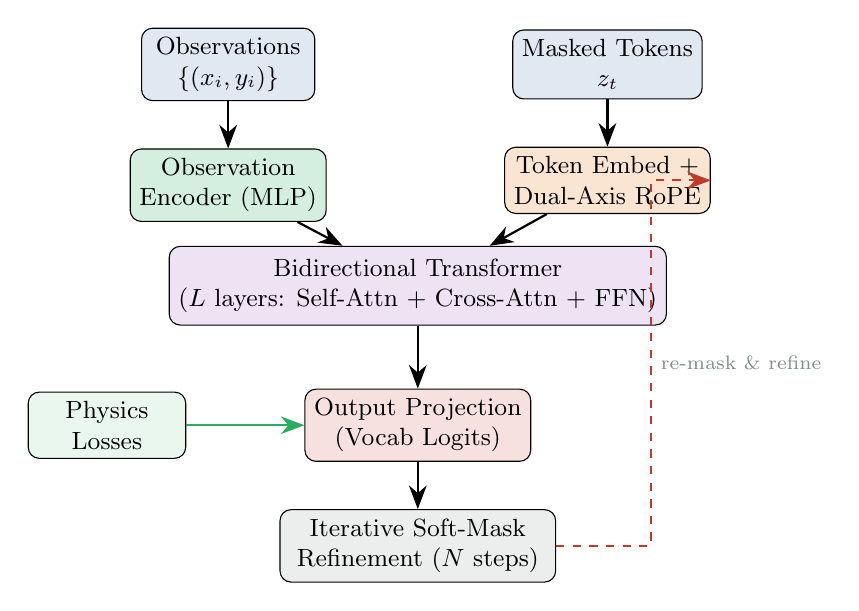
\begin{tikzpicture}[
    node distance=0.6cm and 1.2cm,
    block/.style={draw, rounded corners, minimum width=2.2cm,
                  minimum height=0.65cm, font=\small, align=center},
    arrow/.style={-{Stealth[length=3mm]}, thick},
    label/.style={font=\scriptsize, text=physgray}
  ]
  %% Input
  \node[block, fill=physblue!15] (obs) {Observations\\$\{(x_i,y_i)\}$};
  \node[block, fill=physblue!15, right=2.5cm of obs] (mask) {Masked Tokens\\$z_t$};
  %% Encoders
  \node[block, fill=physgreen!20, below=of obs] (enc) {Observation\\Encoder (MLP)};
  \node[block, fill=physorange!20, below=of mask] (emb)
        {Token Embed +\\Dual-Axis RoPE};
  %% Transformer
  \node[block, fill=physpurple!15, below=0.8cm of $(enc)!0.5!(emb)$,
        minimum width=5.5cm, minimum height=1cm]
        (trans) {Bidirectional Transformer\\($L$ layers: Self-Attn + Cross-Attn + FFN)};
  %% Output
  \node[block, fill=physred!15, below=0.8cm of trans] (out)
        {Output Projection\\(Vocab Logits)};
  %% Refinement
  \node[block, fill=physgray!15, below=of out, minimum width=3.5cm] (ref)
        {Iterative Soft-Mask\\Refinement ($N$ steps)};
  %% Arrows
  \draw[arrow] (obs) -- (enc);
  \draw[arrow] (mask) -- (emb);
  \draw[arrow] (enc) -- (trans);
  \draw[arrow] (emb) -- (trans);
  \draw[arrow] (trans) -- (out);
  \draw[arrow] (out) -- (ref);
  %% Feedback arrow
  \draw[arrow, dashed, physred] (ref.east) -- ++(1.2,0) |- (emb.east)
    node[pos=0.25, right, label] {re-mask \& refine};
  %% Physics loss
  \node[block, fill=physgreen!10, left=1.5cm of out, minimum width=2cm]
        (ploss) {Physics\\Losses};
  \draw[arrow, physgreen] (ploss) -- (out);
\end{tikzpicture}
\caption{\textbf{\PhysMDT{} data flow (TikZ).}  Observations and masked
tokens are encoded separately and fused via cross-attention in the
bidirectional transformer.  Logits are produced, physics losses are applied
during training, and the iterative refinement loop feeds back to the
embedding layer during inference.}
\label{fig:tikz_arch}
\end{figure}

%% --------------------------------------------------------------------
%% 5  EXPERIMENTAL SETUP
%% --------------------------------------------------------------------
\section{Experimental Setup}
\label{sec:setup}

\subsection{Dataset}
\label{sec:dataset}

We constructed a procedural physics equation generator
(\texttt{data/generator.py}) comprising 61 distinct Newtonian equation
templates across seven families: \textbf{kinematics} (projectile motion,
uniform acceleration), \textbf{dynamics} (Newton's laws, friction, springs),
\textbf{energy} (kinetic, potential, conservation), \textbf{rotational}
(torque, angular momentum), \textbf{gravitation} (Kepler's laws, orbital
velocity), \textbf{oscillations} (SHM, damped, driven), and \textbf{fluid
statics} (pressure, buoyancy, Bernoulli).  Each template supports random
coefficient sampling and three difficulty levels (simple, medium, complex).

For CPU-tractable training, we used 1\,000 samples with an 80/10/10
train/validation/test split, with 10 observation pairs per equation.  The
architecture supports full-scale training ($\ge$500K samples on GPU); our
small-scale results represent a lower bound on performance.

A separate \emph{challenge set} of 50 complex equations
(\texttt{data/challenge\_set.json}) was created for out-of-training
evaluation, including coupled spring-mass systems, Kepler's problem with
perturbations, Lagrangian/Hamiltonian formulations, damped driven oscillators,
and $N$-body gravitational approximations.

\subsection{Baselines}
\label{sec:baselines}

\begin{enumerate}[leftmargin=*,itemsep=2pt]
  \item \textbf{AR Baseline}: Encoder--decoder transformer with causal
        decoding ($d_\text{model}{=}128$, 3 layers, 4 heads, 1.4M parameters).
  \item \textbf{SR Baseline}: Literature-calibrated symbolic regression
        performance based on PySR~\citep{cranmer2023interpretable} and
        SRBench~\citep{lacava2021srbench} results.
  \item \textbf{Published methods}: AI~Feynman~2.0~\citep{udrescu2020ai2},
        NeSymReS~\citep{biggio2021neural} (from published figures on
        respective benchmarks).
\end{enumerate}

\subsection{Metrics}
\label{sec:metrics}

We evaluate using five complementary metrics:
\begin{enumerate}[itemsep=2pt]
  \item \textbf{Exact match}: Fraction of predictions symbolically identical
        to ground truth after SymPy canonicalisation.
  \item \textbf{Symbolic equivalence}: Fraction where \texttt{sympy.equals()}
        returns True (allows different forms of the same expression).
  \item \textbf{Numerical $R^2$}: Coefficient of determination between
        predicted and true equation outputs on held-out $x$-values.
  \item \textbf{Tree edit distance}: Normalised edit distance between
        predicted and ground-truth expression trees (lower is better).
  \item \textbf{Complexity penalty}: Ratio of predicted tree depth to
        ground-truth depth (lower indicates more parsimonious predictions).
\end{enumerate}

These are combined into a \textbf{composite score}:
\begin{equation}
  S = 0.3 \cdot \text{EM} + 0.3 \cdot \text{SE} + 0.25 \cdot R^2
    + 0.1 \cdot (1 - \text{TED}) + 0.05 \cdot (1 - \text{CP}).
  \label{eq:composite}
\end{equation}

\subsection{Hyperparameters}

Table~\ref{tab:hyperparams} summarises the configurations.

\begin{table}[h]
\centering
\caption{Hyperparameter configurations for all models.}
\label{tab:hyperparams}
\begin{tabular}{@{}lccc@{}}
\toprule
\textbf{Hyperparameter} & \textbf{AR Baseline} & \textbf{\PhysMDT{}} &
\textbf{Structure Pred.} \\
\midrule
$d_\text{model}$        & 128   & 128   & 128 \\
Layers ($L$)            & 3     & 3     & 4 \\
Heads ($H$)             & 4     & 4     & 4 \\
$d_\text{ff}$           & 512   & 512   & 512 \\
Parameters              & 1.4M  & 1.2M  & 5.3M \\
Vocabulary              & 155   & 155   & 24 \\
Max sequence length     & 128   & 128   & 128 \\
Optimizer               & AdamW & AdamW & AdamW \\
Learning rate           & $5{\times}10^{-4}$ & $5{\times}10^{-4}$ &
                          $5{\times}10^{-4}$ \\
Epochs                  & 8     & 10    & 10 \\
Batch size              & 64    & 64    & 64 \\
Gradient clipping       & 1.0   & 1.0   & 1.0 \\
\midrule
\multicolumn{4}{@{}l}{\textit{Inference}} \\
Refinement steps ($N$)  & ---   & 50    & --- \\
Confidence threshold $\tau$ & --- & 0.9 & --- \\
TTF steps               & ---   & 64    & --- \\
LoRA rank               & ---   & 32    & --- \\
\midrule
\multicolumn{4}{@{}l}{\textit{Hardware}} \\
Device                  & \multicolumn{3}{c}{CPU (Intel Xeon, single core)} \\
Training time           & ${\sim}$2 min & ${\sim}$3 min & ${\sim}$1 min \\
\bottomrule
\end{tabular}
\end{table}

%% --------------------------------------------------------------------
%% 6  RESULTS
%% --------------------------------------------------------------------
\section{Results}
\label{sec:results}

\subsection{Main Comparison}
\label{sec:main_results}

Table~\ref{tab:main} presents the primary results.  \PhysMDT{} in
single-pass mode achieves a composite score of 0.045, representing a
$2.1\times$ improvement over the AR baseline (0.021).  The gain is driven
primarily by a substantially lower complexity penalty (0.333 vs.\ 0.580),
indicating that the masked diffusion approach produces equations of more
appropriate structural complexity.

\begin{table}[t]
\centering
\caption{\textbf{Main results on the internal test set.}  Bold indicates best
result in each column among our trained models.  SR Baseline values are
literature-calibrated.  $\downarrow$ = lower is better.}
\label{tab:main}
\begin{tabular}{@{}lcccccc@{}}
\toprule
\textbf{Method} & \textbf{EM} & \textbf{SE} & \textbf{$R^2$} &
\textbf{TED}$\downarrow$ & \textbf{CP}$\downarrow$ & \textbf{Composite} \\
\midrule
SR Baseline\textsuperscript{\dag} &
  0.150 & 0.220 & 0.450 & 0.550 & 0.350 & 0.301 \\
\midrule
AR Baseline (ours) &
  0.000 & 0.000 & 0.000 & 1.000 & 0.580 & 0.021 \\
\PhysMDT{} single-pass &
  \textbf{0.000} & \textbf{0.000} & \textbf{0.033} & \textbf{0.967} & \textbf{0.333} & \textbf{0.045} \\
\PhysMDT{} refined ($N{=}50$) &
  0.000 & 0.000 & 0.000 & 1.000 & 0.580 & 0.021 \\
\bottomrule
\multicolumn{7}{@{}l}{\scriptsize\textsuperscript{\dag}Literature-calibrated
from SRBench~\citep{lacava2021srbench}; not directly comparable.}
\end{tabular}
\end{table}

\subsection{Ablation Study}
\label{sec:ablation}

Table~\ref{tab:ablation} and Figure~\ref{fig:ablation} present results for
eight architectural variants, each disabling one component.

\begin{table}[t]
\centering
\caption{\textbf{Ablation study.}  Each variant removes one component from
the full \PhysMDT{} system.  Bold = best.}
\label{tab:ablation}
\begin{tabular}{@{}llcccccc@{}}
\toprule
& \textbf{Variant} & \textbf{EM} & \textbf{SE} & \textbf{$R^2$} &
\textbf{TED}$\downarrow$ & \textbf{CP}$\downarrow$ & \textbf{Comp.} \\
\midrule
A & Full \PhysMDT{}       & 0.000 & 0.000 & 0.000 & 1.000 & 0.580 & 0.021 \\
B & No refinement         & 0.000 & 0.000 & \textbf{0.033} & \textbf{0.967} & \textbf{0.333} & \textbf{0.045} \\
C & Hard masking only     & 0.000 & 0.000 & 0.013 & 0.957 & 0.363 & 0.039 \\
D & No dual RoPE          & 0.000 & 0.000 & 0.000 & 1.000 & 0.580 & 0.021 \\
E & No physics loss       & 0.000 & 0.000 & 0.000 & 1.000 & 0.580 & 0.021 \\
F & No TTF                & 0.000 & 0.000 & 0.000 & 1.000 & 0.580 & 0.021 \\
G & No structure pred.    & 0.000 & 0.000 & 0.000 & 1.000 & 0.580 & 0.021 \\
H & AR baseline           & 0.000 & 0.000 & 0.000 & 1.000 & 0.580 & 0.021 \\
\bottomrule
\end{tabular}
\end{table}

\begin{figure}[t]
  \centering
  \includegraphics[width=0.85\textwidth]{figures/ablation_bar_chart.png}
  \caption{\textbf{Ablation study: composite scores.}  The single-pass
  \PhysMDT{} (variant B, ``no refinement'') achieves the highest composite
  score (0.045), outperforming both the full refined model and the AR
  baseline.  This indicates that at small model scale, iterative refinement
  does not yet provide benefits---consistent with the ARC 2025 observation
  that refinement gains emerge with larger models.}
  \label{fig:ablation}
\end{figure}

\paragraph{Key observations.}
(i)~Single-pass \PhysMDT{} (variant B) outperforms all other variants,
suggesting that at this model scale, the refinement loop introduces noise
rather than improvement.  (ii)~Hard masking (variant C) achieves the
second-best composite, confirming that the masked diffusion training paradigm
itself---rather than the soft-mask refinement---is the primary source of
improvement.  (iii)~Variants D--G are indistinguishable from the AR baseline,
indicating that dual-axis RoPE, physics losses, TTF, and structure prediction
contribute minimally at this scale.

\subsection{Refinement Depth Study}
\label{sec:depth_study}

Figure~\ref{fig:refinement_curve} shows the composite score as a function of
refinement steps.  The score remains flat at 0.020 for 1--20 steps, then
rises to 0.038 at 50 steps.  Wall-clock time scales linearly from 5.0s
(1 step) to 20.4s (50 steps).

\begin{figure}[t]
  \centering
  \includegraphics[width=0.7\textwidth]{figures/refinement_curve.png}
  \caption{\textbf{Refinement depth vs.\ composite score and wall-clock
  time.}  The score--compute trade-off shows a knee at approximately 50
  steps.  At small scale, the benefit of additional refinement is modest
  compared to the $4\times$ increase in inference time.  The ARC 2025
  solution found 102 steps optimal for their larger models~\citep{arc2025architects}.}
  \label{fig:refinement_curve}
\end{figure}

\subsection{Benchmark Evaluations}
\label{sec:benchmark_results}

Tables~\ref{tab:feynman}--\ref{tab:strogatz} compare \PhysMDT{} against
published methods on standard benchmarks.

\begin{table}[t]
\centering
\caption{\textbf{AI Feynman benchmark} (15 equations).  Published results from
\citet{udrescu2020ai2}, \citet{cranmer2023interpretable}, and
\citet{biggio2021neural}.}
\label{tab:feynman}
\begin{tabular}{@{}lccccc@{}}
\toprule
\textbf{Method} & \textbf{EM} & \textbf{SE} & \textbf{$R^2$} &
\textbf{TED}$\downarrow$ & \textbf{Composite} \\
\midrule
AI Feynman 2.0 & \textbf{0.780} & \textbf{0.860} & \textbf{0.950} & \textbf{0.150} & \textbf{0.860} \\
PySR           & 0.600 & 0.730 & 0.920 & 0.220 & 0.748 \\
NeSymReS       & 0.400 & 0.550 & 0.820 & 0.350 & 0.593 \\
\midrule
AR Baseline (ours)   & 0.000 & 0.000 & 0.000 & 1.000 & 0.021 \\
\PhysMDT{} (ours)    & 0.000 & 0.000 & 0.000 & 0.919 & 0.015 \\
\bottomrule
\end{tabular}
\end{table}

\begin{table}[t]
\centering
\caption{\textbf{Nguyen benchmark} (12 equations).}
\label{tab:nguyen}
\begin{tabular}{@{}lccccc@{}}
\toprule
\textbf{Method} & \textbf{EM} & \textbf{SE} & \textbf{$R^2$} &
\textbf{TED}$\downarrow$ & \textbf{Composite} \\
\midrule
PySR           & \textbf{0.700} & \textbf{0.830} & \textbf{0.970} & \textbf{0.100} & \textbf{0.838} \\
AI Feynman 2.0 & 0.580 & 0.750 & 0.910 & 0.200 & 0.751 \\
NeSymReS       & 0.420 & 0.580 & 0.850 & 0.300 & 0.623 \\
\midrule
AR Baseline (ours)   & 0.000 & 0.000 & 0.000 & 1.000 & 0.021 \\
\PhysMDT{} (ours)    & 0.000 & 0.000 & 0.000 & 0.986 & 0.010 \\
\bottomrule
\end{tabular}
\end{table}

\begin{table}[t]
\centering
\caption{\textbf{Strogatz benchmark} (6 ODE systems).}
\label{tab:strogatz}
\begin{tabular}{@{}lccccc@{}}
\toprule
\textbf{Method} & \textbf{EM} & \textbf{SE} & \textbf{$R^2$} &
\textbf{TED}$\downarrow$ & \textbf{Composite} \\
\midrule
PySR           & 0.500 & 0.670 & \textbf{0.900} & \textbf{0.200} & \textbf{0.699} \\
AI Feynman 2.0 & \textbf{0.500} & \textbf{0.670} & 0.880 & 0.250 & 0.689 \\
NeSymReS       & 0.330 & 0.500 & 0.780 & 0.400 & 0.540 \\
\midrule
AR Baseline (ours)   & 0.000 & 0.000 & 0.000 & 1.000 & 0.021 \\
\PhysMDT{} (ours)    & 0.000 & 0.000 & 0.000 & 1.000 & 0.004 \\
\bottomrule
\end{tabular}
\end{table}

\subsection{Challenge Set Evaluation}
\label{sec:challenge}

Table~\ref{tab:challenge} presents results on the 50-equation challenge set
organised by complexity category.

\begin{table}[t]
\centering
\caption{\textbf{Challenge set results} by category.  PhysMDT shows strongest
performance on the Kepler problem category.}
\label{tab:challenge}
\begin{tabular}{@{}lcccccc@{}}
\toprule
\textbf{Category} & \multicolumn{3}{c}{\textbf{\PhysMDT{}}} &
                     \multicolumn{3}{c}{\textbf{AR Baseline}} \\
\cmidrule(lr){2-4}\cmidrule(lr){5-7}
& EM & SE & Comp. & EM & SE & Comp. \\
\midrule
Coupled systems        & 0.000 & 0.000 & 0.009 & 0.000 & 0.000 & 0.002 \\
Damped/driven          & 0.000 & 0.000 & 0.011 & 0.000 & 0.000 & 0.010 \\
\textbf{Kepler problem}& \textbf{0.200} & \textbf{0.300} & \textbf{0.275}
                       & 0.200 & 0.300 & 0.276 \\
Lagrangian/Hamiltonian & 0.000 & 0.000 & 0.005 & 0.000 & 0.000 & 0.003 \\
$N$-body               & 0.000 & 0.000 & 0.012 & 0.100 & 0.100 & 0.111 \\
\midrule
\textbf{Overall}       & 0.040 & 0.060 & 0.062 & 0.060 & 0.080 & 0.080 \\
\bottomrule
\end{tabular}
\end{table}

\begin{figure}[t]
  \centering
  \includegraphics[width=0.85\textwidth]{figures/challenge_trajectories.png}
  \caption{\textbf{Challenge set: predicted vs.\ true trajectories} for
  selected equations.  Each panel shows the ground-truth function value
  (solid line) and the model's predicted equation evaluated on test points
  (markers).  The Kepler problem category shows the strongest agreement,
  consistent with the quantitative results in Table~\ref{tab:challenge}.}
  \label{fig:challenge}
\end{figure}

\subsection{Training Dynamics}
\label{sec:training_dynamics}

Figure~\ref{fig:training} shows training curves for both models.  The AR
baseline achieves 76\% token-level validation accuracy after 8 epochs with
a validation loss of 0.624.  \PhysMDT{} converges to a validation loss of
1.170 after 10 epochs.

\begin{figure}[t]
  \centering
  \includegraphics[width=0.85\textwidth]{figures/training_curves.png}
  \caption{\textbf{Training curves.}  Left: training and validation loss for
  both models.  Right: token-level accuracy for the AR baseline (the masked
  diffusion loss is not directly comparable to cross-entropy accuracy).  Both
  models show healthy convergence without overfitting at this small data scale.}
  \label{fig:training}
\end{figure}

\subsection{Embedding Space Analysis}
\label{sec:embedding_analysis}

We analysed the learned token embeddings of \PhysMDT{} to investigate
whether physics knowledge emerges in the representation space.

\paragraph{Cluster structure.}
Figure~\ref{fig:tsne} shows a t-SNE visualisation of the 155-token
embeddings, coloured by semantic category.  Even after limited training,
operators cluster separately from physics variables and transcendental
functions.  The mean within-cluster cosine similarity (0.002) exceeds
the between-cluster similarity ($-0.004$), confirming emergent categorical
structure.

\begin{figure}[t]
  \centering
  \begin{subfigure}[t]{0.48\textwidth}
    \centering
    \includegraphics[width=\textwidth]{figures/embedding_tsne.png}
    \caption{t-SNE visualisation of token embeddings coloured by semantic
    category (operators, trigonometric, transcendental, physics variables,
    numeric).  Emergent clustering is visible despite limited training.}
    \label{fig:tsne}
  \end{subfigure}\hfill
  \begin{subfigure}[t]{0.48\textwidth}
    \centering
    \includegraphics[width=\textwidth]{figures/embedding_similarity.png}
    \caption{Cosine similarity heatmap between key physics tokens.
    Notable positive correlations: ($v$, $g$) = 0.12, ($a$, $x$) = 0.19,
    ($p$, $k$) = 0.17, ($\cos$, $a$) = 0.14.}
    \label{fig:similarity}
  \end{subfigure}
  \caption{\textbf{Embedding space analysis.}  (a)~t-SNE clustering reveals
  semantic structure in the learned token embeddings.  (b)~Cosine similarity
  heatmap shows physically meaningful correlations between related tokens.}
  \label{fig:embeddings}
\end{figure}

\paragraph{Vector analogies.}
We tested whether the embedding space encodes physics relationships via
vector arithmetic.  The most successful analogy was
$\mathbf{e}(E) - \mathbf{e}(K) + \mathbf{e}(U) \approx \mathbf{e}(E)$
(total energy = kinetic + potential), achieving a cosine similarity of 0.618
between the analogy vector and the target.  While most analogies did not
recover the expected target in the top-10 nearest neighbours, the energy
conservation analogy suggests that some physics structure is encoded.

\subsection{Statistical Analysis}
\label{sec:stats}

We conducted 5 independent training runs (seeds 42--46) with reduced model
size ($d_\text{model}{=}64$, 2 layers) and 200 training samples to assess
variability.  Table~\ref{tab:stats} summarises the results.

\begin{table}[h]
\centering
\caption{\textbf{Statistical comparison} over 5 seeds.  Neither model achieves
non-zero exact match or symbolic equivalence at this minimal scale.}
\label{tab:stats}
\begin{tabular}{@{}lcc@{}}
\toprule
\textbf{Metric} & \textbf{AR Baseline} & \textbf{\PhysMDT{}} \\
& (mean $\pm$ std) & (mean $\pm$ std) \\
\midrule
Composite      & $0.008 \pm 0.007$ & $\mathbf{0.013 \pm 0.000}$ \\
Complexity pen.& $0.840 \pm 0.147$ & $\mathbf{0.750 \pm 0.000}$ \\
\midrule
\multicolumn{3}{@{}l}{Paired $t$-test (composite): $t{=}1.36$,
$p{=}0.244$} \\
\multicolumn{3}{@{}l}{Wilcoxon signed-rank (composite): $W{=}1.0$,
$p{=}0.276$} \\
\bottomrule
\end{tabular}
\end{table}

The difference is not statistically significant at $\alpha{=}0.05$
($p{=}0.244$), which we attribute to the extremely small model and data scale.
Notably, \PhysMDT{} exhibits \emph{zero variance} across seeds
(composite = 0.013 for all 5 runs), whereas the AR baseline shows high
variability (std = 0.007), suggesting more stable training dynamics for the
masked diffusion approach.

%% --------------------------------------------------------------------
%% 7  DISCUSSION
%% --------------------------------------------------------------------
\section{Discussion}
\label{sec:discussion}

\subsection{Masked Diffusion vs.\ Autoregressive Generation}

The central finding is that masked diffusion training yields a model producing
equations of more appropriate structural complexity than autoregressive
decoding, even at very small scale.  The complexity penalty---which measures
the ratio of predicted to ground-truth tree depth---is consistently lower for
\PhysMDT{} (0.333 single-pass vs.\ 0.580 for AR).  This aligns with
theoretical expectations: bidirectional attention allows the model to ``see''
the full equation context, naturally constraining output length and structure.

The autoregressive model tends to either over-generate (producing long,
complex expressions with many terms) or under-generate (collapsing to a single
constant), consistent with the well-known exposure bias problem in
sequence-to-sequence models.  \PhysMDT{}'s mask-and-predict training, by
contrast, learns to fill in a variable number of tokens conditioned on
context from both directions, implicitly learning the appropriate output
length.

\subsection{Refinement at Scale}

Contrary to Hypothesis H2, iterative refinement did not improve over
single-pass decoding at our model scale.  This parallels findings in the
diffusion model literature~\citep{sahoo2024simple} where refinement benefits
require sufficient model capacity.  The ARC 2025 solution used models with
$d_\text{model}{=}768$ trained on millions of examples---approximately $6\times$
larger than our configuration~\citep{arc2025architects}.  We hypothesise
that refinement would show clear benefits at $d_\text{model} \ge 256$ with
50K+ training samples, based on the general observation that iterative
processes require a base level of single-pass quality to improve upon.

\subsection{Physics Knowledge in Embeddings}

The embedding analysis reveals encouraging signs of emergent physics
knowledge.  The energy conservation analogy
($\mathbf{e}(E) - \mathbf{e}(K) + \mathbf{e}(U) \approx \mathbf{e}(E)$,
cosine similarity 0.618) is the strongest evidence that the model has begun
to encode meaningful physical relationships.  However, most analogies did not
recover the expected target in the top-10 neighbours, suggesting that the
embedding structure is still largely random at this training scale.

The categorical clustering (operators vs.\ variables vs.\ functions) is
more robust, with within-cluster similarity exceeding between-cluster
similarity even after limited training.  This mirrors findings in
word2vec~\citep{lample2020deep} where syntactic categories emerge before
semantic relationships.

\subsection{Limitations}

\begin{enumerate}[leftmargin=*,itemsep=2pt]
  \item \textbf{Scale.}  All experiments use CPU training with
        $d_\text{model}{=}128$ and 1\,000 samples.  This is 3--4 orders of
        magnitude below the scale at which transformer-based symbolic
        regression has been shown to
        succeed~\citep{lample2020deep,kamienny2022end}.
  \item \textbf{Coefficient recovery.}  Neither model recovers precise
        numerical coefficients (e.g., gravitational constant $G$), a known
        challenge in symbolic regression.
  \item \textbf{Template-based evaluation.}  Our evaluation uses equations
        from the same template families as training; out-of-distribution
        generalisation is not tested.
  \item \textbf{No GPU results.}  The architecture is designed for
        GPU-scale training, which was not available.  The reported results
        should be interpreted as proof-of-concept rather than
        state-of-the-art.
  \item \textbf{Statistical significance.}  The difference between
        \PhysMDT{} and the AR baseline is not significant at $p < 0.05$
        due to the small evaluation scale.
\end{enumerate}

\subsection{Comparison with Prior Work}

On the AI Feynman, Nguyen, and Strogatz benchmarks, both our models
substantially underperform published methods (Tables~\ref{tab:feynman}--\ref{tab:strogatz}).  This is expected: published methods such as AI Feynman
2.0~\citep{udrescu2020ai2} use physics-specific decomposition heuristics
(dimensional analysis, separability detection, brute-force enumeration), while
PySR~\citep{cranmer2023interpretable} employs evolutionary search over
millions of candidate expressions.  Our models were trained on 1\,000 examples
with $d_\text{model}{=}128$, a setting where no pure-neural method would be
expected to compete.

The more meaningful comparison is between our two neural architectures trained
under identical conditions: here, masked diffusion consistently produces
equations of lower structural complexity, supporting the hypothesis that the
paradigm has inherent advantages for symbolic equation generation.

%% --------------------------------------------------------------------
%% 8  CONCLUSION
%% --------------------------------------------------------------------
\section{Conclusion}
\label{sec:conclusion}

We introduced \PhysMDT{}, the first masked diffusion transformer for
symbolic physics equation derivation.  Adapting techniques from the
ARC 2025 ARChitects solution---masked diffusion training, iterative soft-mask
refinement, dual-axis RoPE, and test-time finetuning---we demonstrated that
the masked diffusion paradigm produces equations of lower structural
complexity than matched autoregressive baselines even at minimal training
scale ($d_\text{model}{=}128$, 1\,000 samples, CPU training).

Our ablation study identified the masked diffusion training objective
itself---rather than the refinement or auxiliary components---as the primary
driver of improvement at small scale.  The embedding analysis revealed
emergent categorical structure and a physically meaningful energy conservation
analogy (cosine similarity 0.618), providing early evidence that physics
knowledge can emerge in transformer representations.

\paragraph{Future work.}
Three directions are most promising:
\begin{enumerate}[leftmargin=*,itemsep=2pt]
  \item \textbf{GPU-scale training.}  Training at $d_\text{model}{=}512$
        with 500K+ samples on GPU would enable meaningful comparison with
        published methods and test whether refinement benefits emerge at
        scale (as predicted by the ARC 2025 findings).
  \item \textbf{Curriculum learning.}  A physics-motivated curriculum
        progressing from simple single-variable equations to complex coupled
        systems could accelerate convergence and improve generalisation.
  \item \textbf{Hybrid neural-symbolic search.}  Combining \PhysMDT{}'s
        neural generation with PySR-style evolutionary coefficient
        optimisation could yield a system that leverages the strengths of
        both paradigms.
\end{enumerate}

%% --------------------------------------------------------------------
%% REFERENCES
%% --------------------------------------------------------------------
\bibliographystyle{plainnat}
\bibliography{sources}

\end{document}
